\section{Definition of Gem}
For completeness we briefly recall the basic definitions of gem theory, leading to its definition, \cite{lins1995gca}.
A {\em 4-graph} $G$ is a finite bipartite 4-regular graph whose edges are partitioned into 4 colors,
0,1,2, and 3, 
so that at each vertex there is an edge of each color, a proper edge-coloration, \cite{bondy1976gta}.
For each $i \in \{0,1,2,3\}$, let $E_i$ denote the set of $i$-colored edges of $G$.
A $\{j,k\}$-residue in a $4$-graph $G$ is a connected component of the subgraph induced by $E_j \cup E_k$.
A 2-residue is a $\{j,k\}$-residue, for some distinct colors $j$ and $k$.
A {\em gem} is a 4-graph $G$ such that for each color $i$, $G\backslash E_i$ can be embedded in the plane 
such that the boundary of each face is a 2-residue. From a gem there exists a straightforward
algorithm to obtain a closed orientable 3-manifold, in two different, dual ways. Every such a manifold is obtainable in this way.
An unecessary big gem is obtained from a triangulation $T$ for a manifold by taking the dual of the 
barycentric subdivision of $T$. Here the colors corresponds to the dimensions. Doing simplifications in the gem
completely destroys this correspondence.


\section{Wings as seeds for obtaining the dual PL-complex $\mathcal{H}_n^\star$}

This is the third of 3 closely related articles.
References for the companion papers are \cite{linsmachadoA2012} and \cite{linsmachadoB2012}.

Let $\Pi_\ell$  ($\Pi_r$) be the half plane limited by the $z$-axis 
which contains $a_1=z_0z_2/2$ $(b_1=z_1z_2/2)$.
The construction of the wings and nervures of the next section are exemplified in Figs. \ref{fig:winglist01} to \ref{fig:winglist11}.

\subsection{Wings: reformulating a difficult 3D-problem 
into an easy planar one}\label{subsec:wings}

At some point in our research it became evident that what was needed to obtain the PL-complex $\mathcal{H}_n^\star$ 
was a proper embedding into $\mathbb{R}^3$ of the set of 0-simplices $\{a_1, a_2,\ldots,a_f\} \cup \{b_1, b_2,\ldots,b_g\}$.
The other 0-simplices are obtained by bisections of segments linking previously defined points. It came as a surprise to discover
that this apparently difficult 3D problem was reformulated as a plane problem for which we had at hand an easy solution,
namely Tutte's barycentric method.

We construct a 
sequence of pairs of plane
graphs $\{\{\mathcal{W}^\ell_1,\mathcal{W}^r_1\},
\{\mathcal{W}^\ell_2,\mathcal{W}^r_2\},\ldots,
\{\mathcal{W}^\ell_n,\mathcal{W}^r_n\} \}.$ The $m$-th such pair
constitutes the {\em left} and {\em right wings} \index{wings} of the colored $2$-complex
$\mathcal{H}_m^\star$. The left wings are embedded into $\Pi_\ell$ and
the right wings are embedded into $\Pi_r$. 
We define $\mathcal{W}^\ell_1$ as the set of $2n$ straight line segments
$a_1z_3^1, a_1z_3^2, \ldots, a_1z_3^{2n} \subseteq \Pi_\ell$,
and $\mathcal{W}^\ell_1$ as the set of $2n$ straight line segments
$b_1z_3^1, b_1z_3^2, \ldots, b_1z_3^{2n}  \subseteq \Pi_r$.
The {\em outer triangular region of the left wings} is the plane region
spanned by $a_1, z_3^1,z_3^{2n}$. The {\em outer triangular region of 
the right wings} is the plane region spanned by
$b_1, z_3^1, z_3^{2n}$. 
The passage from $\{\mathcal{W}^\ell_{m-1},\mathcal{W}^r_{m-1}\}$
to $\{\mathcal{W}^\ell_m,\mathcal{W}^r_m\}$ in the $(m-1)$-th $bp$-move,
which we call a {\em $wbp$-move}, corresponds
in $(\mathcal{H}_{m-1}, \mathcal{H}_{m})$ to either a 
0-flip that subdivides a 13-gon into two (case
where the tail of the balloon is of color 0)
or else to a 1-flip that subdivides a 03-gon into two (case
where the tail of the balloon's is of color 1).  
At this point, we need to define a tree called the \index{nervure of a wing} {\em nervure of a wing}.
This is done inductively.
The first ones, $\mathcal{W}^\ell_1$ and $\mathcal{W}^r_1$ have, respectively 
the degenerated trees formed by single points $a_1$ and $b_1$ as their nervures.
In the unique wing that changes with the $bp$-move, a vertex $x_\ell$ corresponding
to either a 13-gon or else to a 03-gon (in a way to be made clear in the poof of
Lemma \ref{lem:internalpointsbigons}).
The intersection of the balloon's head and 
its tail in $\mathcal{H}^\star_m$ is a PL1-face formed by two
simplices meeting at a point $a_p$ (if the tail of the balloon is of color 1)
or $b_q$, if it is of color 0. 
Along the process we define the following auxiliary functions, with arguments
%$1 \le m \le n-1$ or
 $1 \le m \le n-1$:  
$c(m),u(m),v(m),r(m),s(m),
\ell_a(m), \ell_b(m), t_a(m), t_b(m).$
The color
of the $m$-th balloon's tail is denoted by $c(m) \in \{0,1\}$.
Let $u(m), v(m)$ be the odd and even indices of the $m$-th 
balloon's head $\nabla_{u(m)} \cup \nabla_{v(m)}$. 
Let $r(m), s(m)$ be the odd and even indices of the $m$-th 
balloon's tail given by the PL2$_{c(m)}$-face $\subseteq 
\nabla_{r(m)} \cap \nabla_{s(m)}$.
The positive integers $\ell_a(m)$ and $\ell_b(m)$ are the last $a$- and $b$-indices
in left $m$-th wing and right $m$-th wing, respectively.
Indices $p$ or $q$ in the $m$-th $bp$-move satisfy $p=t_a(m)$ or $q=t_b(m)$.
In the passage $\mathcal{H}_m^\star$ to $\mathcal{H}_{m+1}^\ast$ either 
vertex $a_p$ is replaced by $a_{p'},A_p,a_{p''}$, where $p'=\ell_a(m)+1$ and 
$p'' =\ell_a(m)+2$ or else
$b_q$ is replaced by $b_{q'},B_p,b_{q''}$, where $q'=\ell_b(m)+1$ and $q''=\ell_b(m)+2$,
depending on the color of the balloon's tail. In the first case, we add two new edges
$a_{p'}A_p$ and $a_{p''}A_p$ to the nervure, in the second case, we add the edges
$b_{q'}B_p$ and $b_{q''}B_q$ to the nervure. In both cases, $p''=p'+1$ or
$q''=q'+1$. In the pictures the edges of the nervure
are thicker than the ones in the respective wing.
For $1\le m\le n$, and $h\in \{\ell,r\}$, the nervure of $\mathcal{W}^h_m$, 
denoted $\mathcal{N}^h_m$, is a spanning tree of the graph 
$\mathcal{W}^h_m \cup \mathcal{N}^h_m \backslash Z$, where $Z= \{z_3^j~|~ j\in \{1, \ldots, 2n\}\}.$
See Fig. \ref{fig:controlmaps01}, Fig. \ref{fig:controlmaps01novo1},  
Fig. \ref{fig:controlmaps01novo2}
and the complete sequence of figures for the $r^{24}_5$-example, 
Figs. \ref{fig:winglist01}-\ref{fig:winglist11}. 
A vertex in the tree $\mathcal{N}^h_m$ is {\em pendant} if it has degree at most 1.



\begin{lemma}
 Let $1\le m \le n$. The set of pendant vertices of $\mathcal{N}_m^\ell$ is
in 1-1 correspondence with the set of 13-gons of $\mathcal{H}_m$. 
 The set of pendant vertices in $\mathcal{N}_m^r$ is
in 1-1 correspondence with the 03-gons of $\mathcal{H}_m$.
\label{lem:internalpointsbigons}
\end{lemma}
\begin{proof}
The intersection of the $(m-1)$-th balloon's head and tail is a 
PL1-face with two 1-simplices. Their intersection is a point in $\Pi_h$.
The PL1-face dualy corresponds to a 13-gon (resp. 03-gon) in $\mathcal{H}_{m-1}$
if $h=\ell$ ($h=r$). After the 0-flip (resp. 1-flip) that produces  $\mathcal{H}_m$
the PL1-face is splitted into two, in a conformal way with the passage 
from  $\mathcal{W}^h_{m-1} \cup \mathcal{N}^h_{m-1}$ to  
$\mathcal{W}^h_m \cup \mathcal{N}^h_m$. Given this interpretation
the Lemma is easily established by induction.
\end{proof}


%--------------------
\begin{figure}[!htb]
\begin{center}
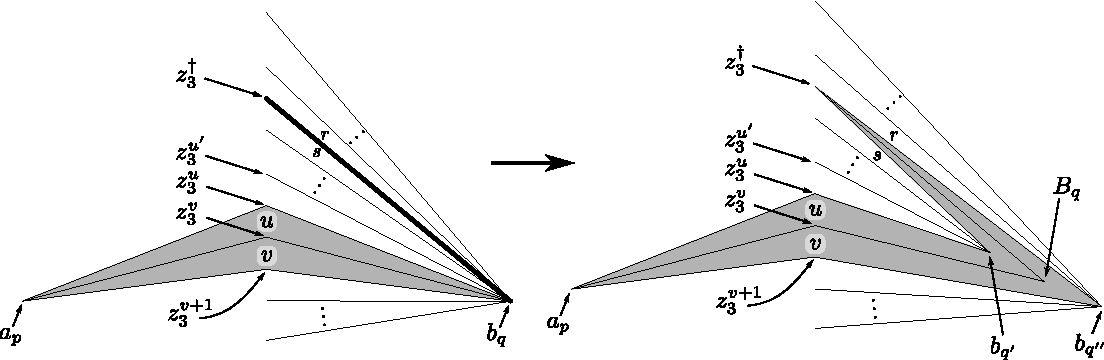
\includegraphics[width=15.4cm]{A.figs/controlmaps01.pdf}
\caption{$wbp$-move: balloon's head section is painted in gray, 
and the part of balloon's tail that is intersecting the appropriate
semi-plane is depicted as a {\em thick edge}. \index{thick edge}}
\label{fig:controlmaps01}
\end{center}
\end{figure}
%--------------------

\begin{figure}[!htb]
\begin{center}
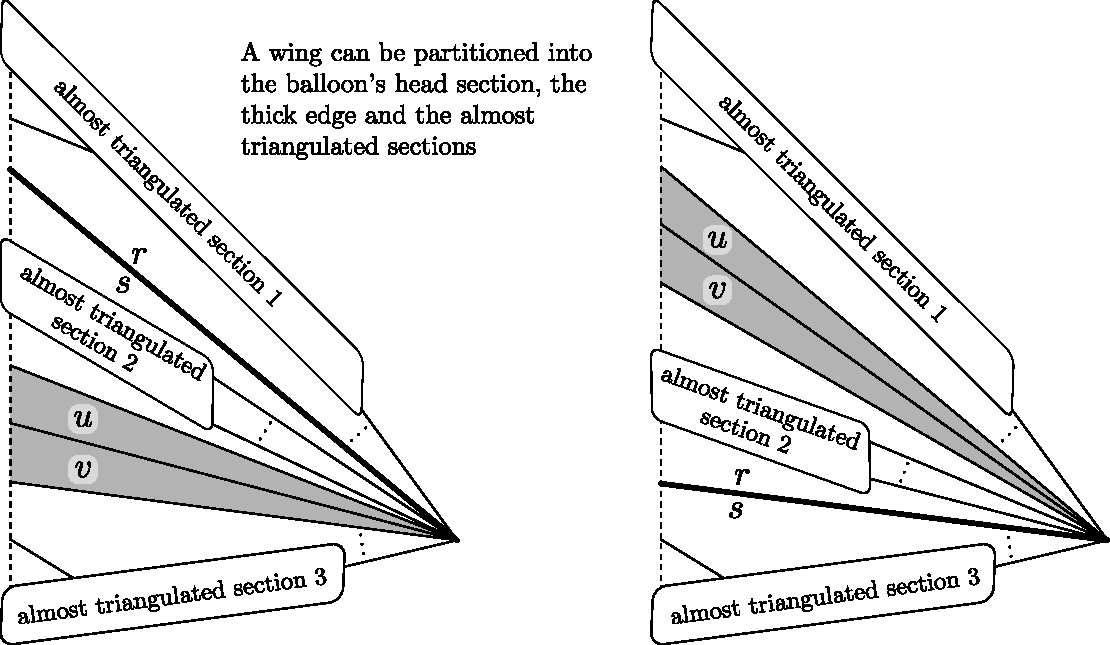
\includegraphics[width=15cm]{A.figs/controlmaps01novo1.pdf}
\caption{Given a half-wing and a balloon it can be partitioned into the 
balloon's head section, thick edge and
some {\em almost triangulated} sections.}
 %meaning that some faces are bounded by plane quadrilaterals instead of triangles.}
\label{fig:controlmaps01novo1}
\end{center}
\end{figure}

\begin{figure}[!htb] 
\begin{center}
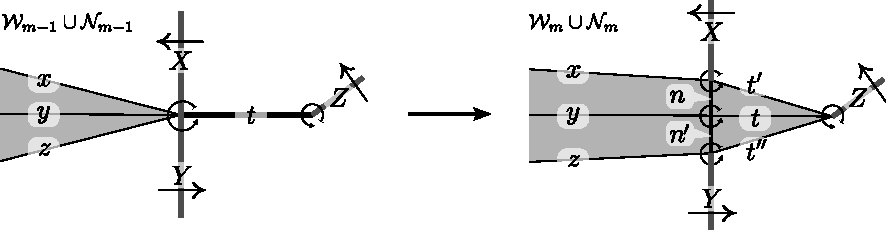
\includegraphics[width=15 cm]{A.figs/controlmaps01novo2.pdf}
\caption{The {\em star} \index{star} of a vertex of a graph embedded in a surface is the counterclockwise cyclic sequence of 
edges incident to the vertex (such an ordering is induced by the surface).
The set of stars is called a { \em rotation} \index{rotation} and has the 
characterizing property that each edge appears twice.
The general case of changing rotation when going from 
$\mathcal{W}_{\ell-1} \cup \mathcal{N}_{\ell-1}$ to
$\mathcal{W}_{\ell} \cup \mathcal{N}_{\ell}$ is depicted above. 
The rotation completely specifies the topological embedding.}
\label{fig:controlmaps01novo2}
\end{center}
\end{figure}

A graph is {\em rectilinearly embedded into $\mathbb{R}^3$} if 
the images of their edges are straight
line segments.
It is a straightforward application of Tutte's barycentric method \cite{tutte1963dg},
\cite{colin2003tutte} to obtain a rectilinear embedding of
$\mathcal{W}_n^h \cup \mathcal{N}_n^h$ which fixes the vertices in the boundary of the 
outer triangular region of $\Pi_h$, $h \in \{\ell,r\}$.
Tutte's method has an intrinsic connection with the Laplacian of graphs, see  \cite{Klarreich0412}.
We rotate $\Pi \in \{ \Pi_\ell, \Pi_r \}$
so that it becomes the $xz$-plane. After having the planar coordinates
$\Pi_h$ is rotated back to its initial position and we have the 
$\mathcal{W}_n^h \cup \mathcal{N}_n^h$ rectilinearly embedded into $\mathbb{R}^3$.
Tutte's method becomes very efficient because of Lemma \ref{lem:numberofedges}.


Tutte's method suffers of the clustering problem where vertices accumulate
in some small regions. Even though theoretically this is not 
needed, we present a heuristic of attaching weights to the edges
to improve the result. An edge with weight $k\in\mathbb{N}$ behaves
as $k$ parallel edges.
We define the weights for the edges of the wings as 1.
If the edge is in the nervure,
to calculate the weight, we use the whole wing. 
Start defining these weights as 0, so from leaves to root, 
define the weight of an edge
as the weight of the vertex incident to it and closer to 
the leaves minus 1, Fig. \ref{fig:arvorecompesos}.
In Fig. \ref{fig:controlmapsnovo6} we compare the two results,
without and with weights given by three times the weights in the nervure 
of Fig. \ref{fig:arvorecompesos}, 
for obtaining the final left wing of the $r^{24}_5$-example.


Tutte's method is applied twice: to plane graphs $\mathcal{W}_n^\ell \cup \mathcal{N}_n^\ell$ and to $\mathcal{W}_n^r \cup \mathcal{N}_n^r.$
In each application we use $O(n)$ iterations to solve a linear system in $\mathbb{C}$. This is theoretically sufficient
to achive rectilineatiry (which nevertheless can be verified). As each one of the plane graphs has less than $6n-4$ edges by Lemma \ref{lem:numberofedges}, 
the total time to obtain $\mathcal{W}_n^\ell \cup \mathcal{W}_n^r$ embedded into $\Pi_\ell \cup \Pi_r$ is $O(n^2)$.

\begin{lemma}\label{lem:numberofedges}
 The number of edges of $\mathcal{W}_n^h \cup \mathcal{N}_n^h$, $h \in \{\ell,r\}$
is at most $6n-4$.
\end{lemma}
\begin{proof}
The number of 1-simplices in the left wing and in the right wing of the 
initial complex in the sequence are both $2n$. At each one of the $n-1$ $bp$-moves
we add 4 edges either to the left or to the right wing with its nervure.
Thus each one of the final left and right wings with nervures has at most $6n-4$ edges.
\end{proof}

\begin{figure}[!htb]
\begin{center}
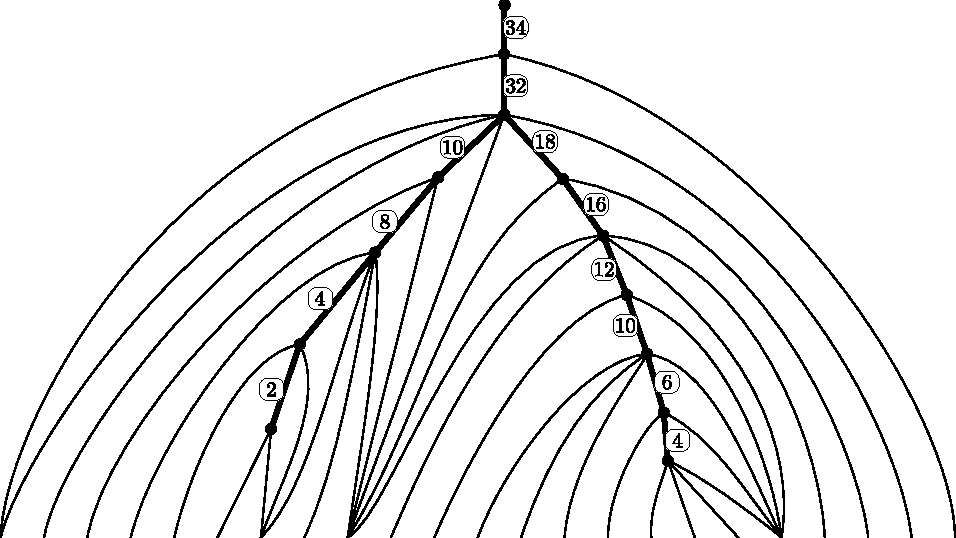
\includegraphics[width=13cm]{A.figs/arvorecompesos.pdf}
\caption{Computing the weights for Tutte's barycentric method via the wing nervure.}
\label{fig:arvorecompesos}
\end{center}
\end{figure}

\begin{figure}[!htb]
\begin{center}
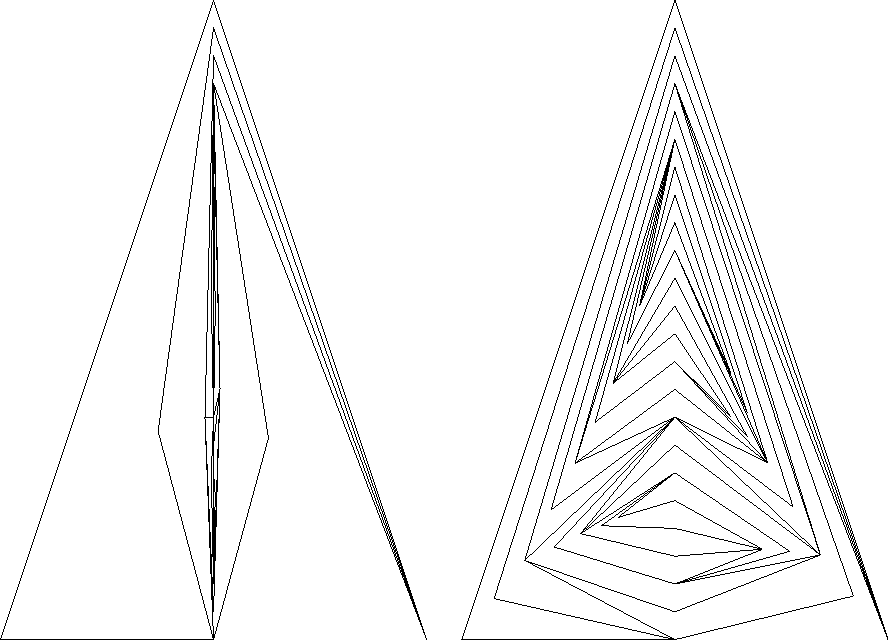
\includegraphics[width=13cm]{A.figs/controlmapsnovo6.pdf}
\caption{Tutte's embbeding without and with the weights (final pair of 
wings without nervure for the $r_5^{24}$-example).}
\label{fig:controlmapsnovo6}
\end{center}
\end{figure}
%\begin{lemma} 
%\label{theo:containement}
%$$\mathcal{U}^\star_n \subseteq (z_0 \ast W_n^\ell) 
%\cup (z_2 \ast W_n^\ell) \cup (z_1 \ast W_n^r) \cup (z_2 \ast W_n^r) 
%\bigcup_{i=1}^{2n} (z_3^i \ast z_0z_1) .$$
%\end{lemma}
%\begin{proof}
%Every 2-simplex of $\mathcal{U}^\star_m$ is contained in one of the 4+2n cones.
%\end{proof}

